
\documentclass[UTF8]{ctexart}
\usepackage[T1]{fontenc}
\usepackage{amsmath}
\usepackage{graphicx}
\usepackage{mathdots}
\setlength{\parindent}{0em}
\begin{document}
\section{1}
分配率  A+BC=(A+B)(A+C)  \\
P(A$\bar{B}$)=P(A)-P(AB) \\
X Y 独立 $\rightarrow$ $X^2  Y^2$ 独立 \\
A B 独立 $\rightarrow A \bar{B} ; \bar{A} \bar{B} $ 独立 \\
$\sum_{i=0}^k C_m^i C_n^{k-i}=C_{m+n}^k$ \\
A-B=A-AB=A$\bar{B}$ \\
$C\subset AB \longrightarrow \overline{C} \supset \overline{A} \cup \overline{B} $ \\
$ES^2=DX$;
$DS^2=\frac{2\sigma^4}{n-1}$ \\
相合估计  \\  \mbox{二阶中心距} $\frac{1}{n} \sum_{i=1}^nX_i^2 \rightarrow EX^2  \\ \mbox{一阶中心距}    \bar{x}=\frac{1}{n}\sum_{i=1}^nX_i \rightarrow EX$
样本方差是$\sigma^2$的无偏估计量 \\
二阶样本中心距$\frac{n-1}{n}S^2$是$\sigma^2$的最大似然估计量 \\
$S^2$是$\sigma^2$的相合估计量 \\

\section{协方差}
$D(X\pm Y)=DX+DY \pm 2Cov(X,Y)$ \\
Cov(X,c)=0 ;  Cov(aX+b,Y)=aCov(X,Y) \\ $Cov(X_1+X_2,Y)=Cov(X_1,Y)+Cov(X_2,Y)$ \\
Cov(x,y)=E[(X-EX)(Y-EY)]=EXY-EX$\cdot$EY \\

$\rho_{xy}=\frac{Cov(X,Y)}{\sqrt{DX}\sqrt{DY}}$

\section{正态分布}
X~N(0,1) E|X|=$\sqrt{\frac{2}{\pi}}$

\section{二维正态分布}
$f(x,y)=\frac{1}{2 \pi \sigma_1 \sigma_2 \sqrt {1- \rho ^2 }}exp
\left\{
 - \frac{1}{2(1- \rho^2)}
\left[
 {(\frac{x- \mu_1}{\sigma_1})}^2
 -2 \rho
 (\frac{x- \mu_1}{\sigma_1})
 (\frac{y-\mu_2}{\sigma_2})
 +{(\frac{y-\mu_2}{\sigma_2})}^2
 \right]
 \right\}
$
\section{相互独立的随机变量分布}
\subsection{和}
$Z=X+Y \longrightarrow f_z(z)=\int_{-\infty}^{+\infty}f(x,z-x)dx=\int_{-\infty}^{+\infty}f(z-y,y)dy$ \\
\subsection{差}
$Z=X-Y \longrightarrow f(z)=\int_{-\infty}^{+\infty}f(x,x-z)dx=\int_{-\infty}^{+\infty}f(x+z,x)dx$
\subsection{积}
$Z=XY \longrightarrow f_z(z) = \int_{-\infty}^{+\infty}
\frac{1}{|x|}
f(x,\frac{z}{x})
dx=
\int_{-\infty}^{+\infty}
\frac{1}{|y|}
f(\frac{z}{y},{y})
dy
$
\subsection{商}
$Z=\frac{X}{Y} \longrightarrow
f_z(z)=
\int_{-\infty}^{+\infty}
|y|
f(yz,y)
dy
$
\section{切比雪夫}
DX 存在
$\epsilon>0
\rightarrow P\{|X-EX|\geq \epsilon\}\leq\frac{DX}{\epsilon^2} ;
P\{|X-EX|< \epsilon\}\geq1-\frac{DX}{\epsilon^2}$
\section{估计量}
$\sigma^2$的最大似然估计量$\frac{1}{n}
\sum_{i=1}^n
{(X_i - \bar{x})}^2$

\section{数理统计}
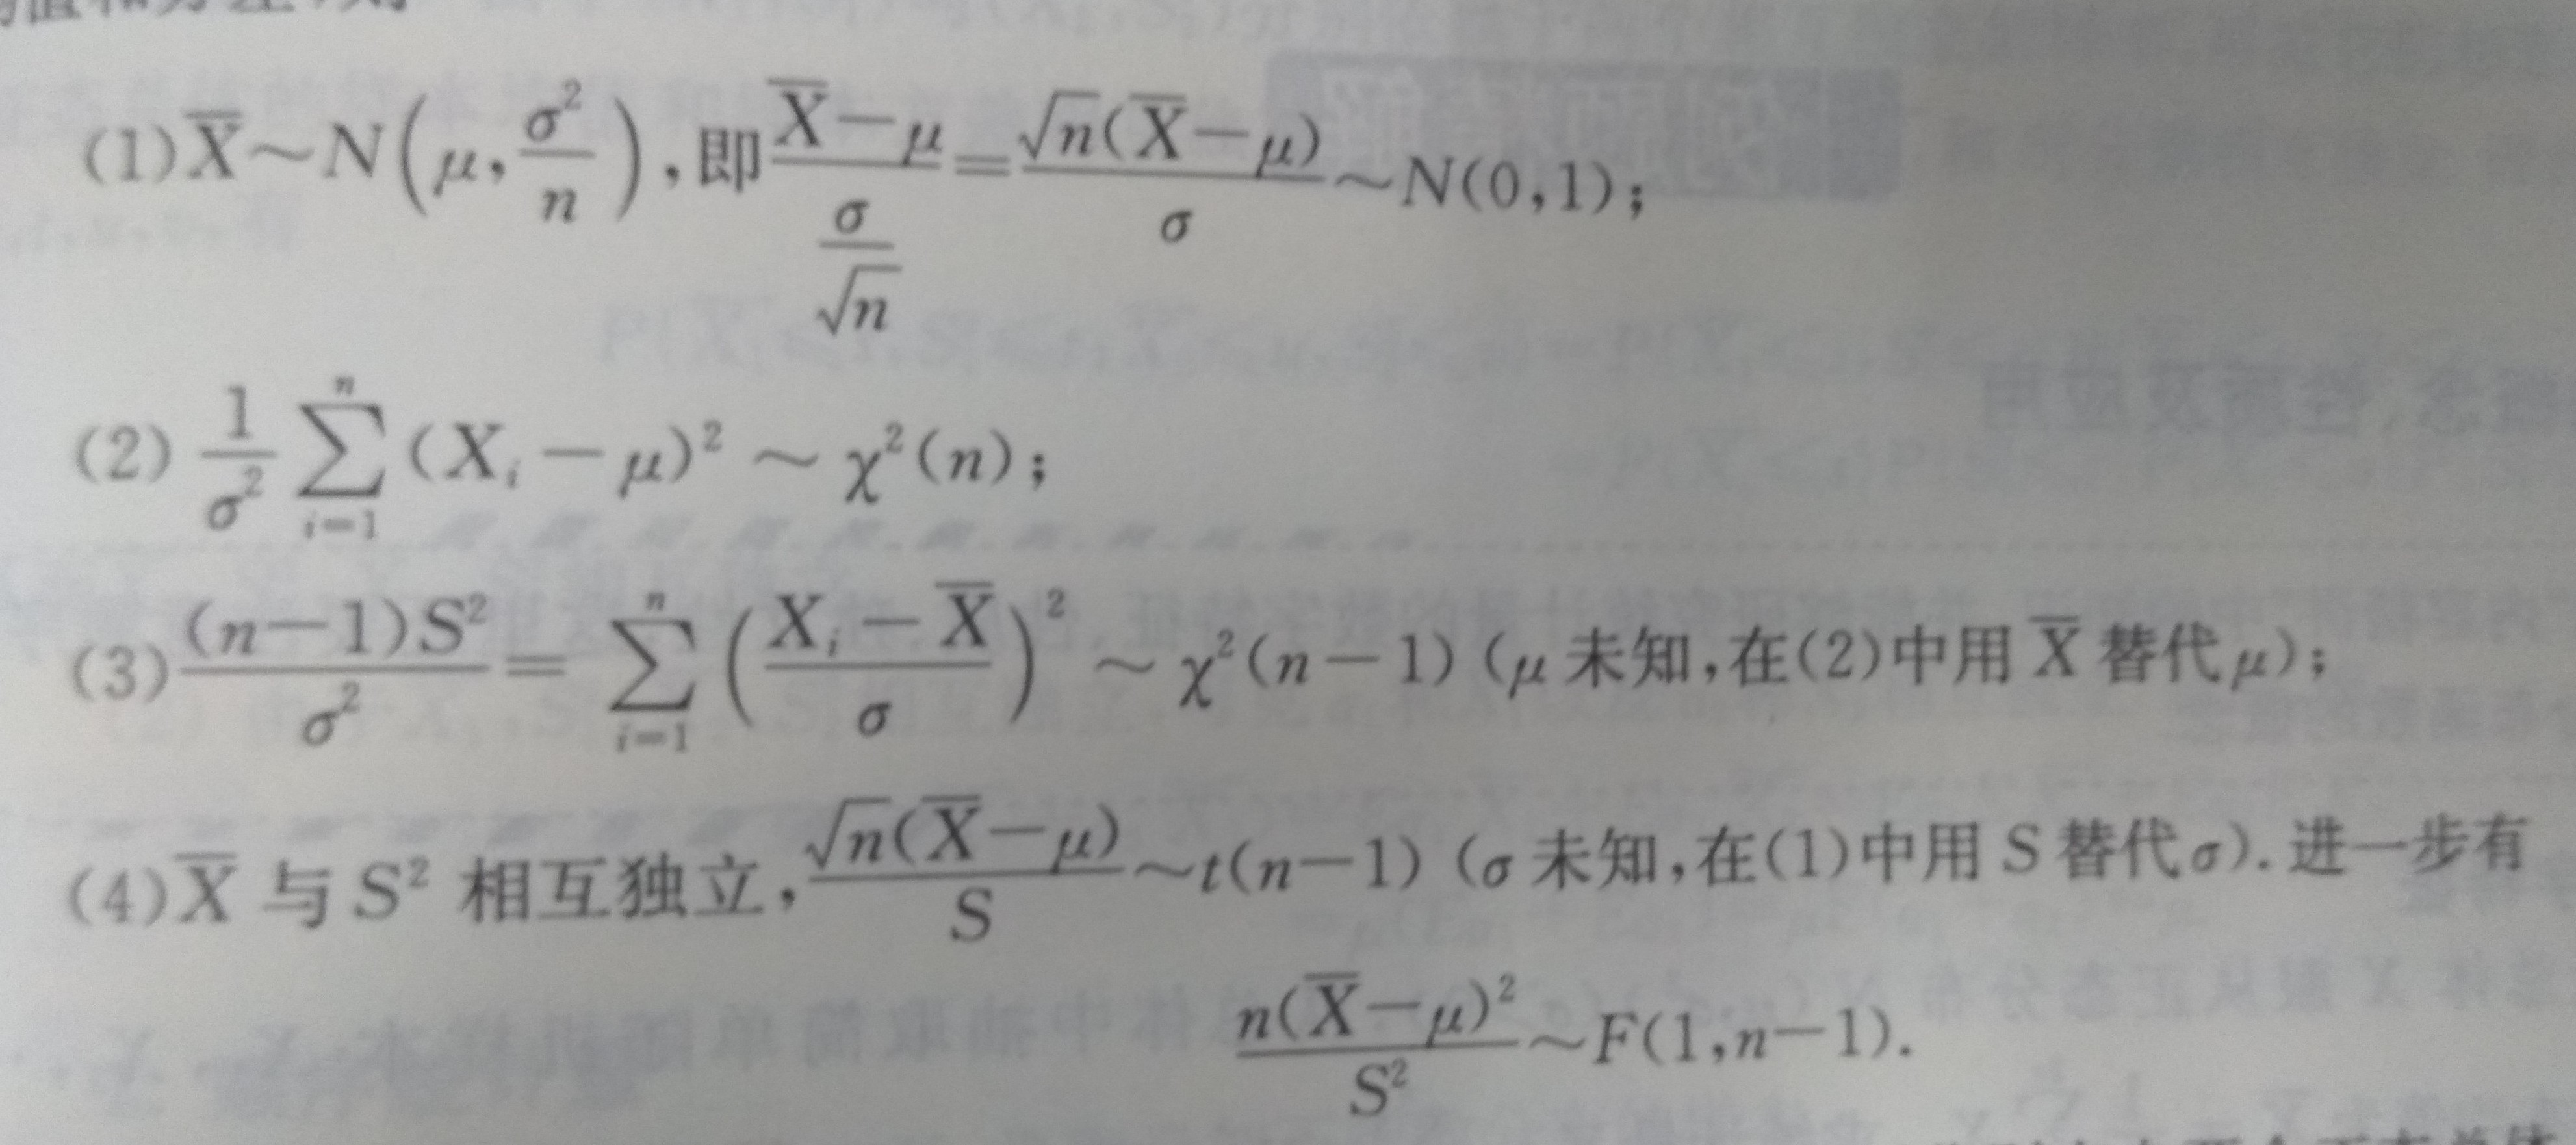
\includegraphics[width=15cm]{9345E7/danzhengtai.jpg}
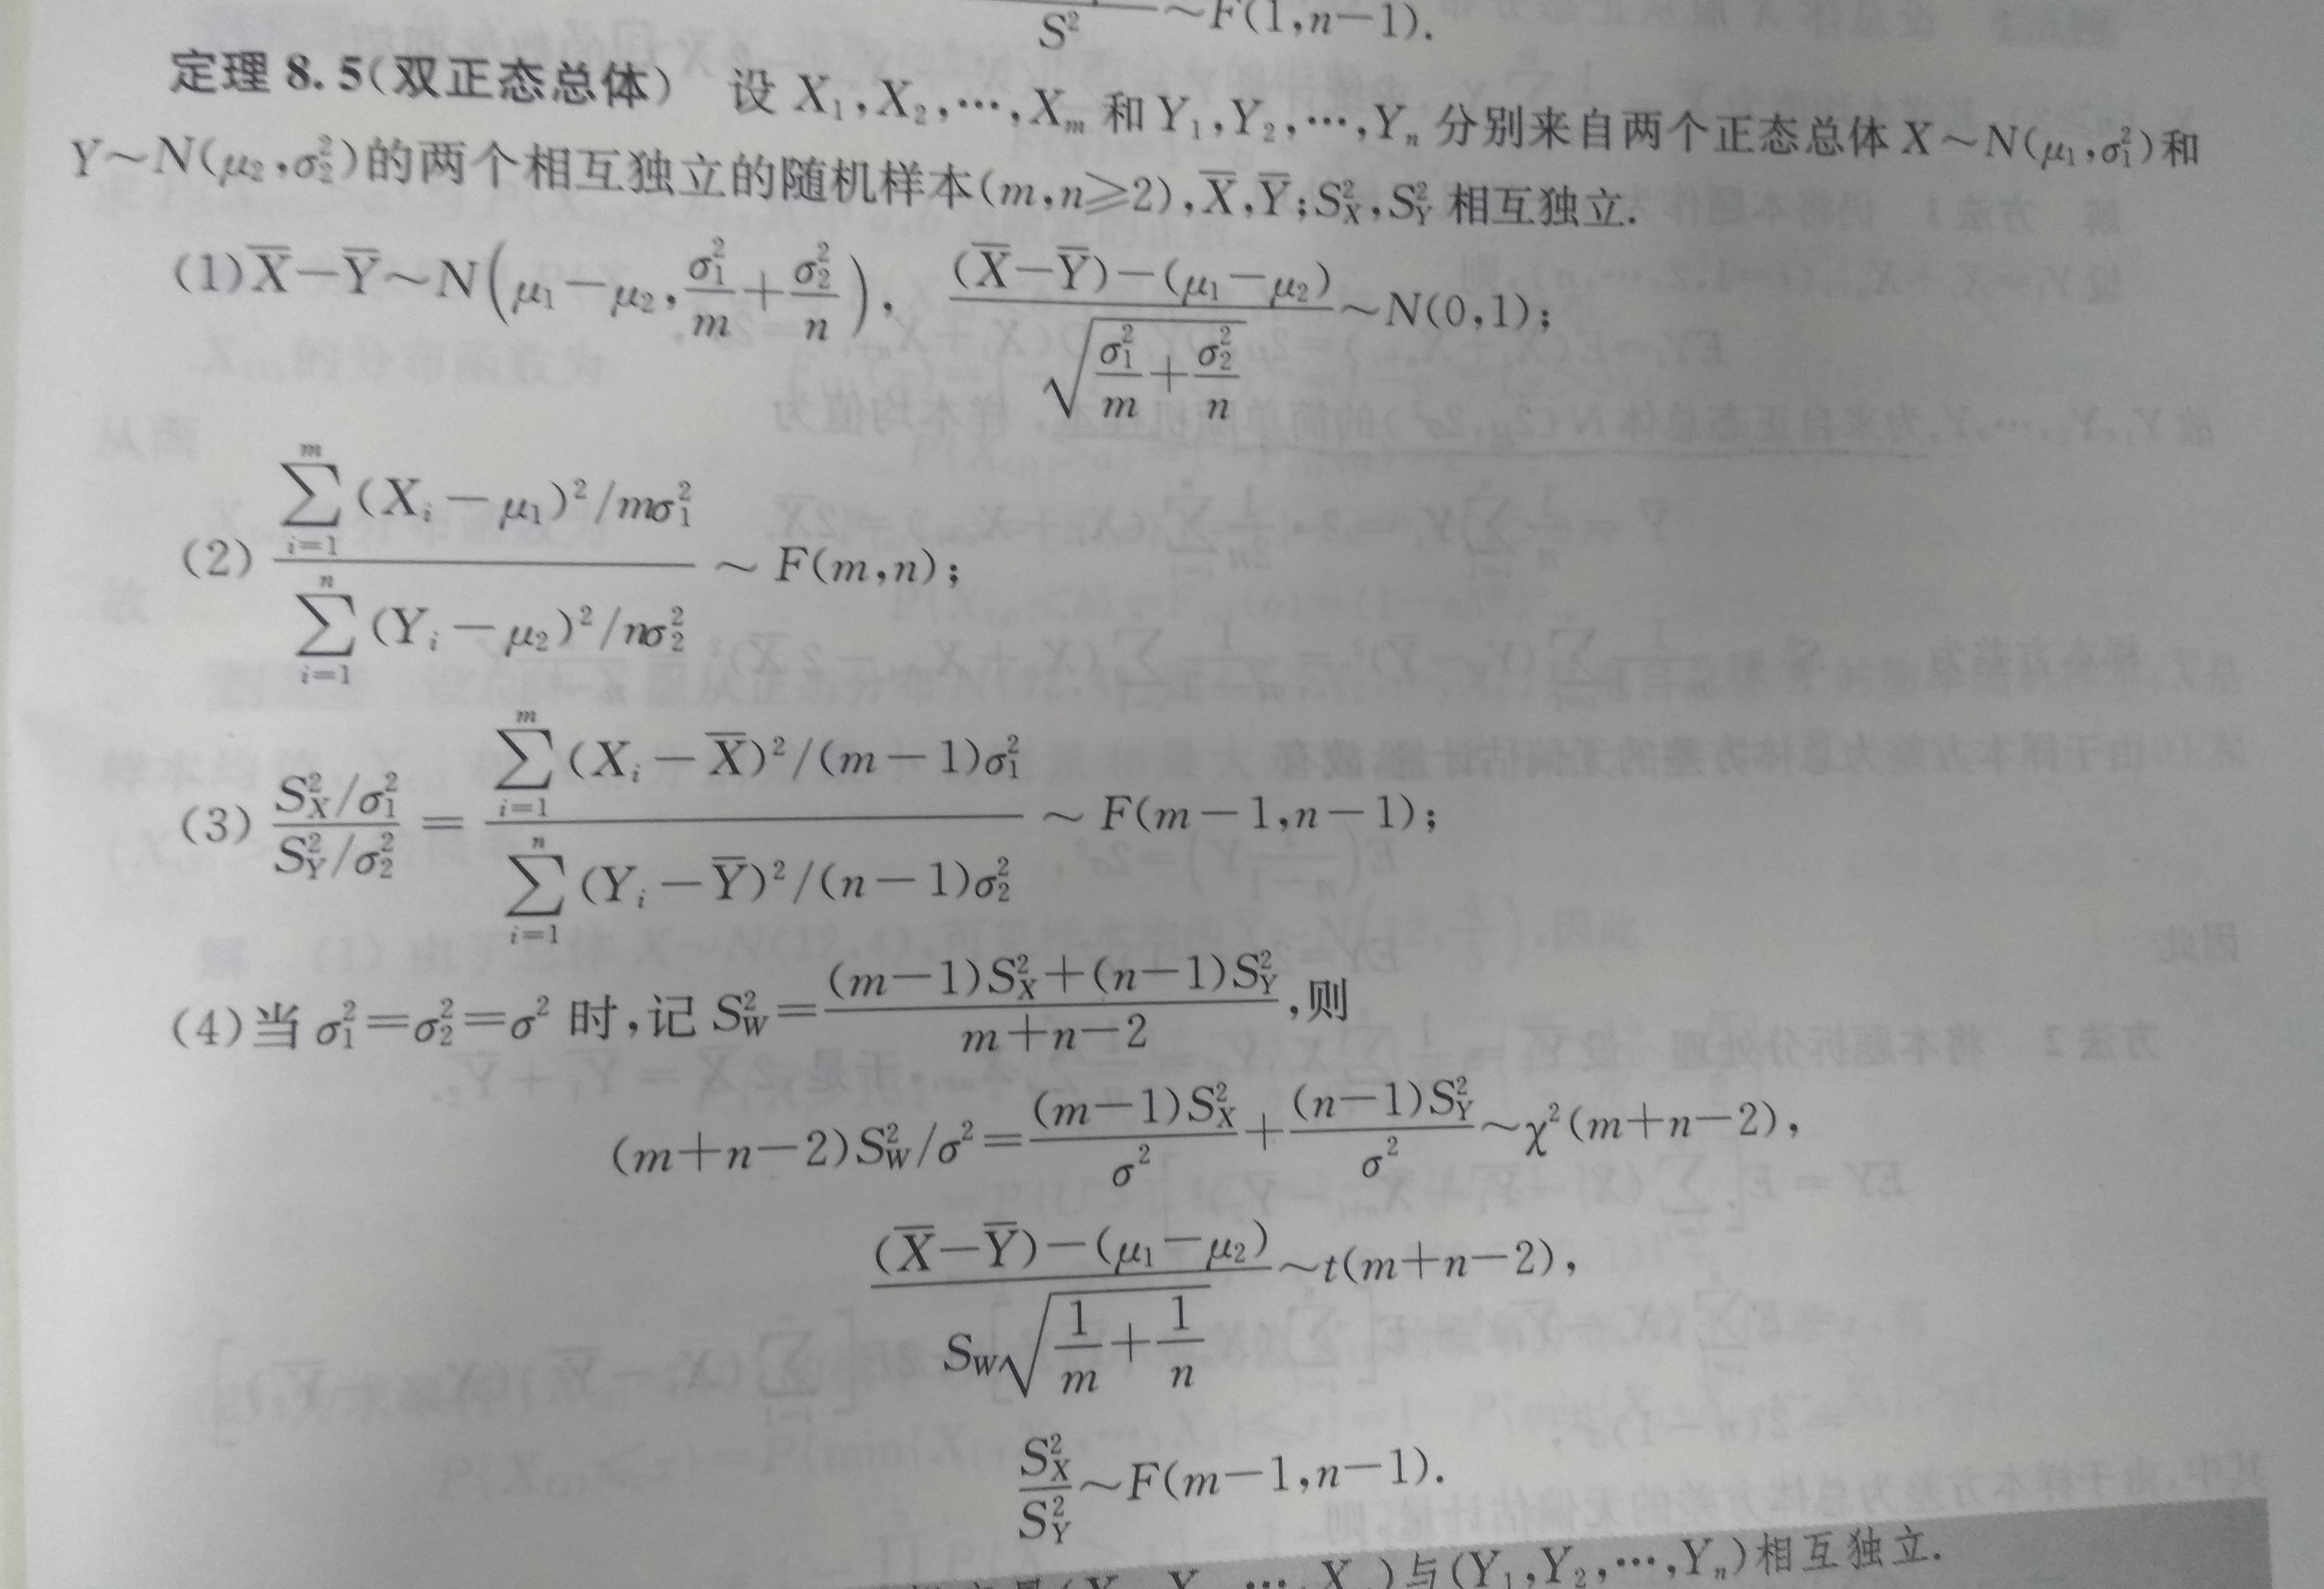
\includegraphics[width=15cm]{9345E7/shuangzhengtai.jpg}
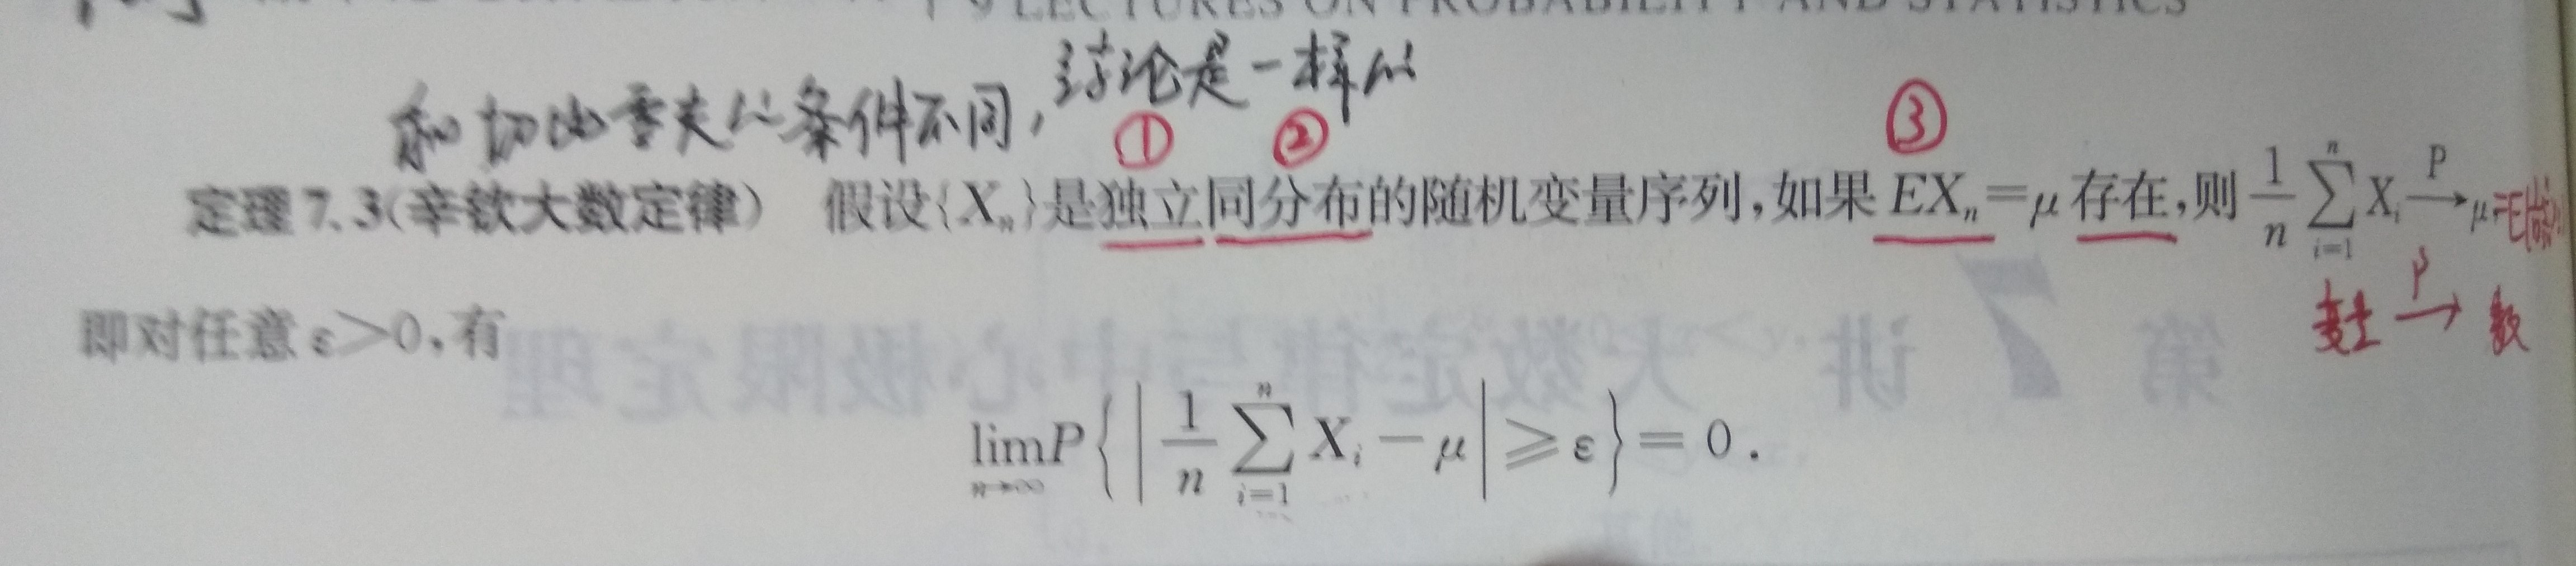
\includegraphics[width=15cm]{9345E7/xinqin.jpg}
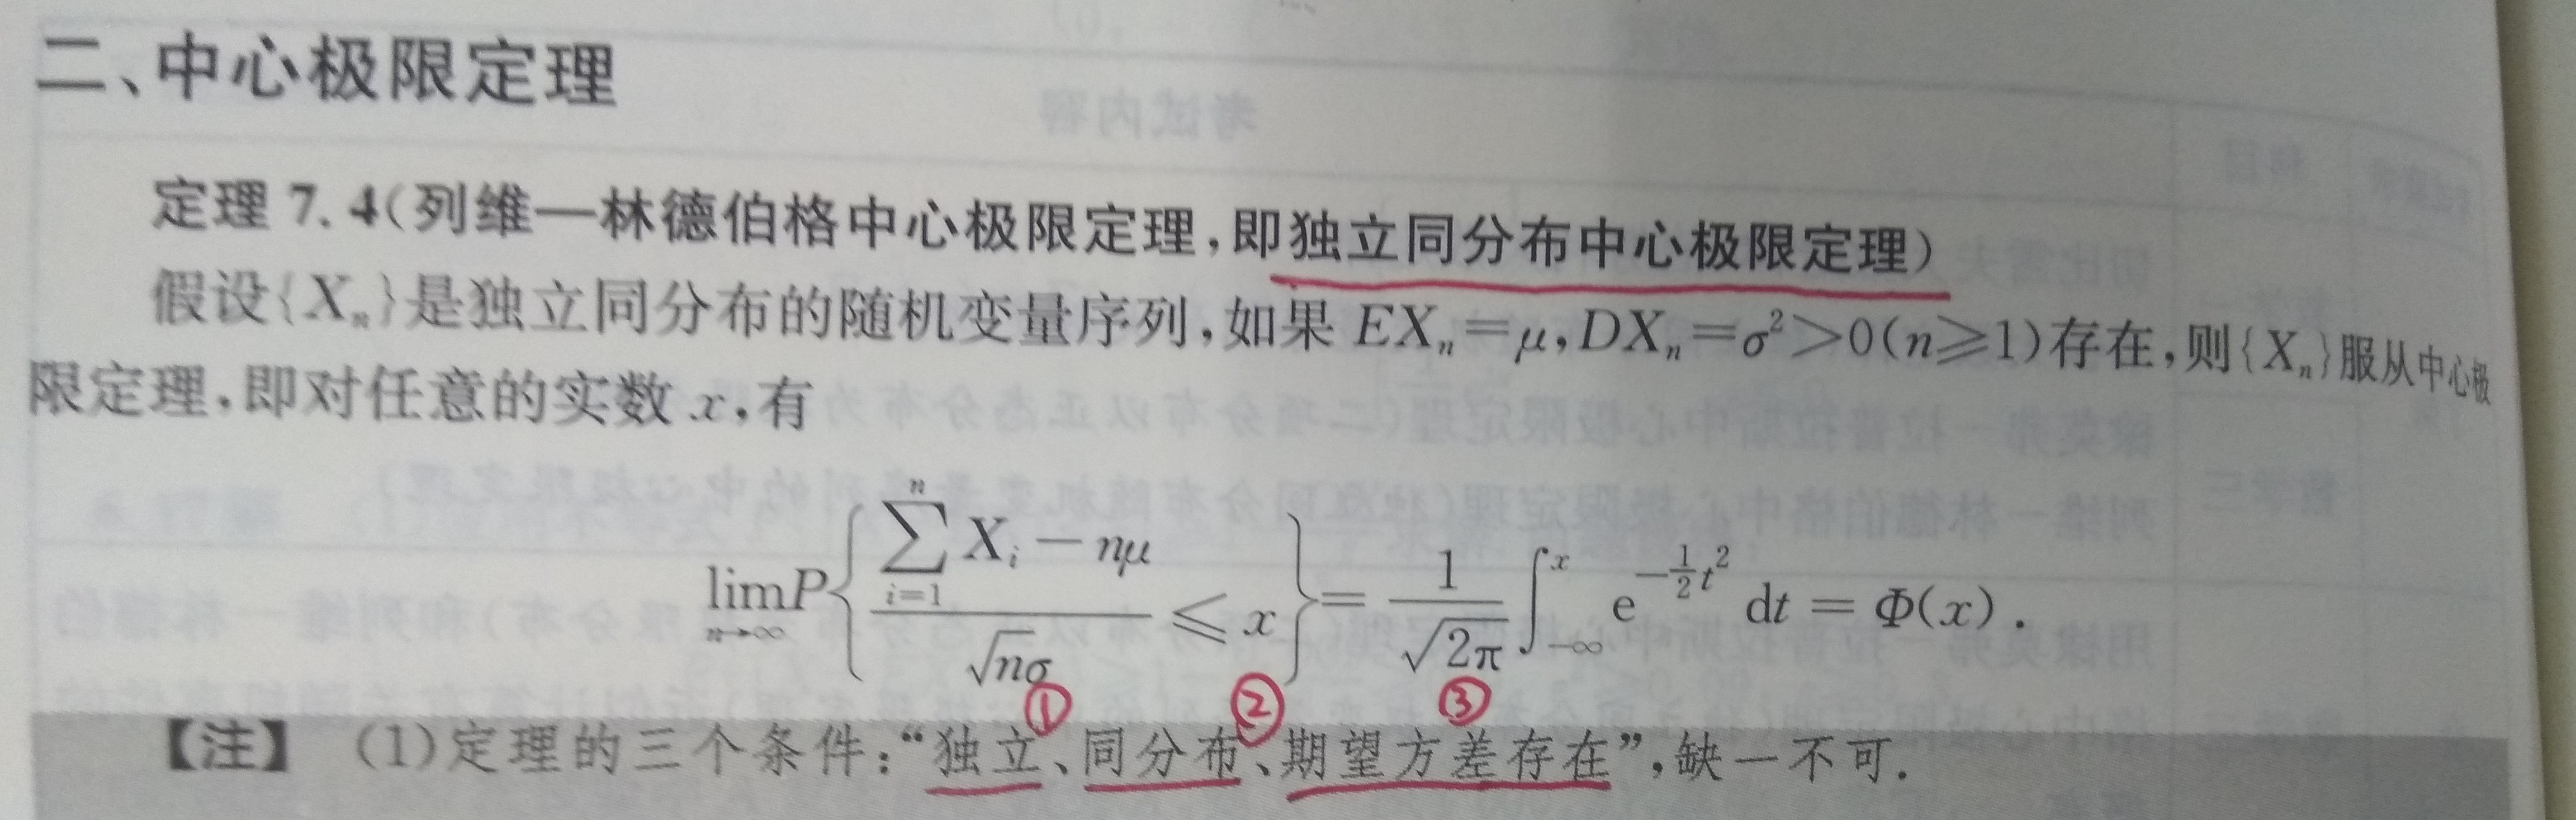
\includegraphics[width=15cm]{9345E7/zhongxinjixian.jpg}

\end{document}
